\textit{La phase d'analyse est un élément indispensable à la bonne réalisation du projet. Dans un premier temps, les fonctionnalités de l'application y sont décrites et caractérisées, notamment à l'aide d'un diagramme UML de cas d'utilisations. Une seconde partie présente les étapes successives qui nous ont permis d'arriver à la modélisation finale, sous la forme de diagrammes UML de classes et de \og{}discussions\fg{}.}

Discours sur tous les schéma UML (usecases, class).

Discussion des choix des diag de classe.

Fini par le choix final justifié !

\section{Fonctionnalités}

L'application devra modéliser un thésaurus stocké dans une base de données, et devra permettre sa consultation au travers d'une interface web. L'utilisateur pourra donc consulter ou administrer les données. La consultation du thésaurus se fera donc par navigation dans un vue hiérarchique ou par nœud. Un outil de recherche facilitera l'accès aux données. Le module d'administration permettra quand à lui d'ajouter, de modifier et de supprimer les termes et les concepts, ainsi que les relations.

\begin{figure}[H]
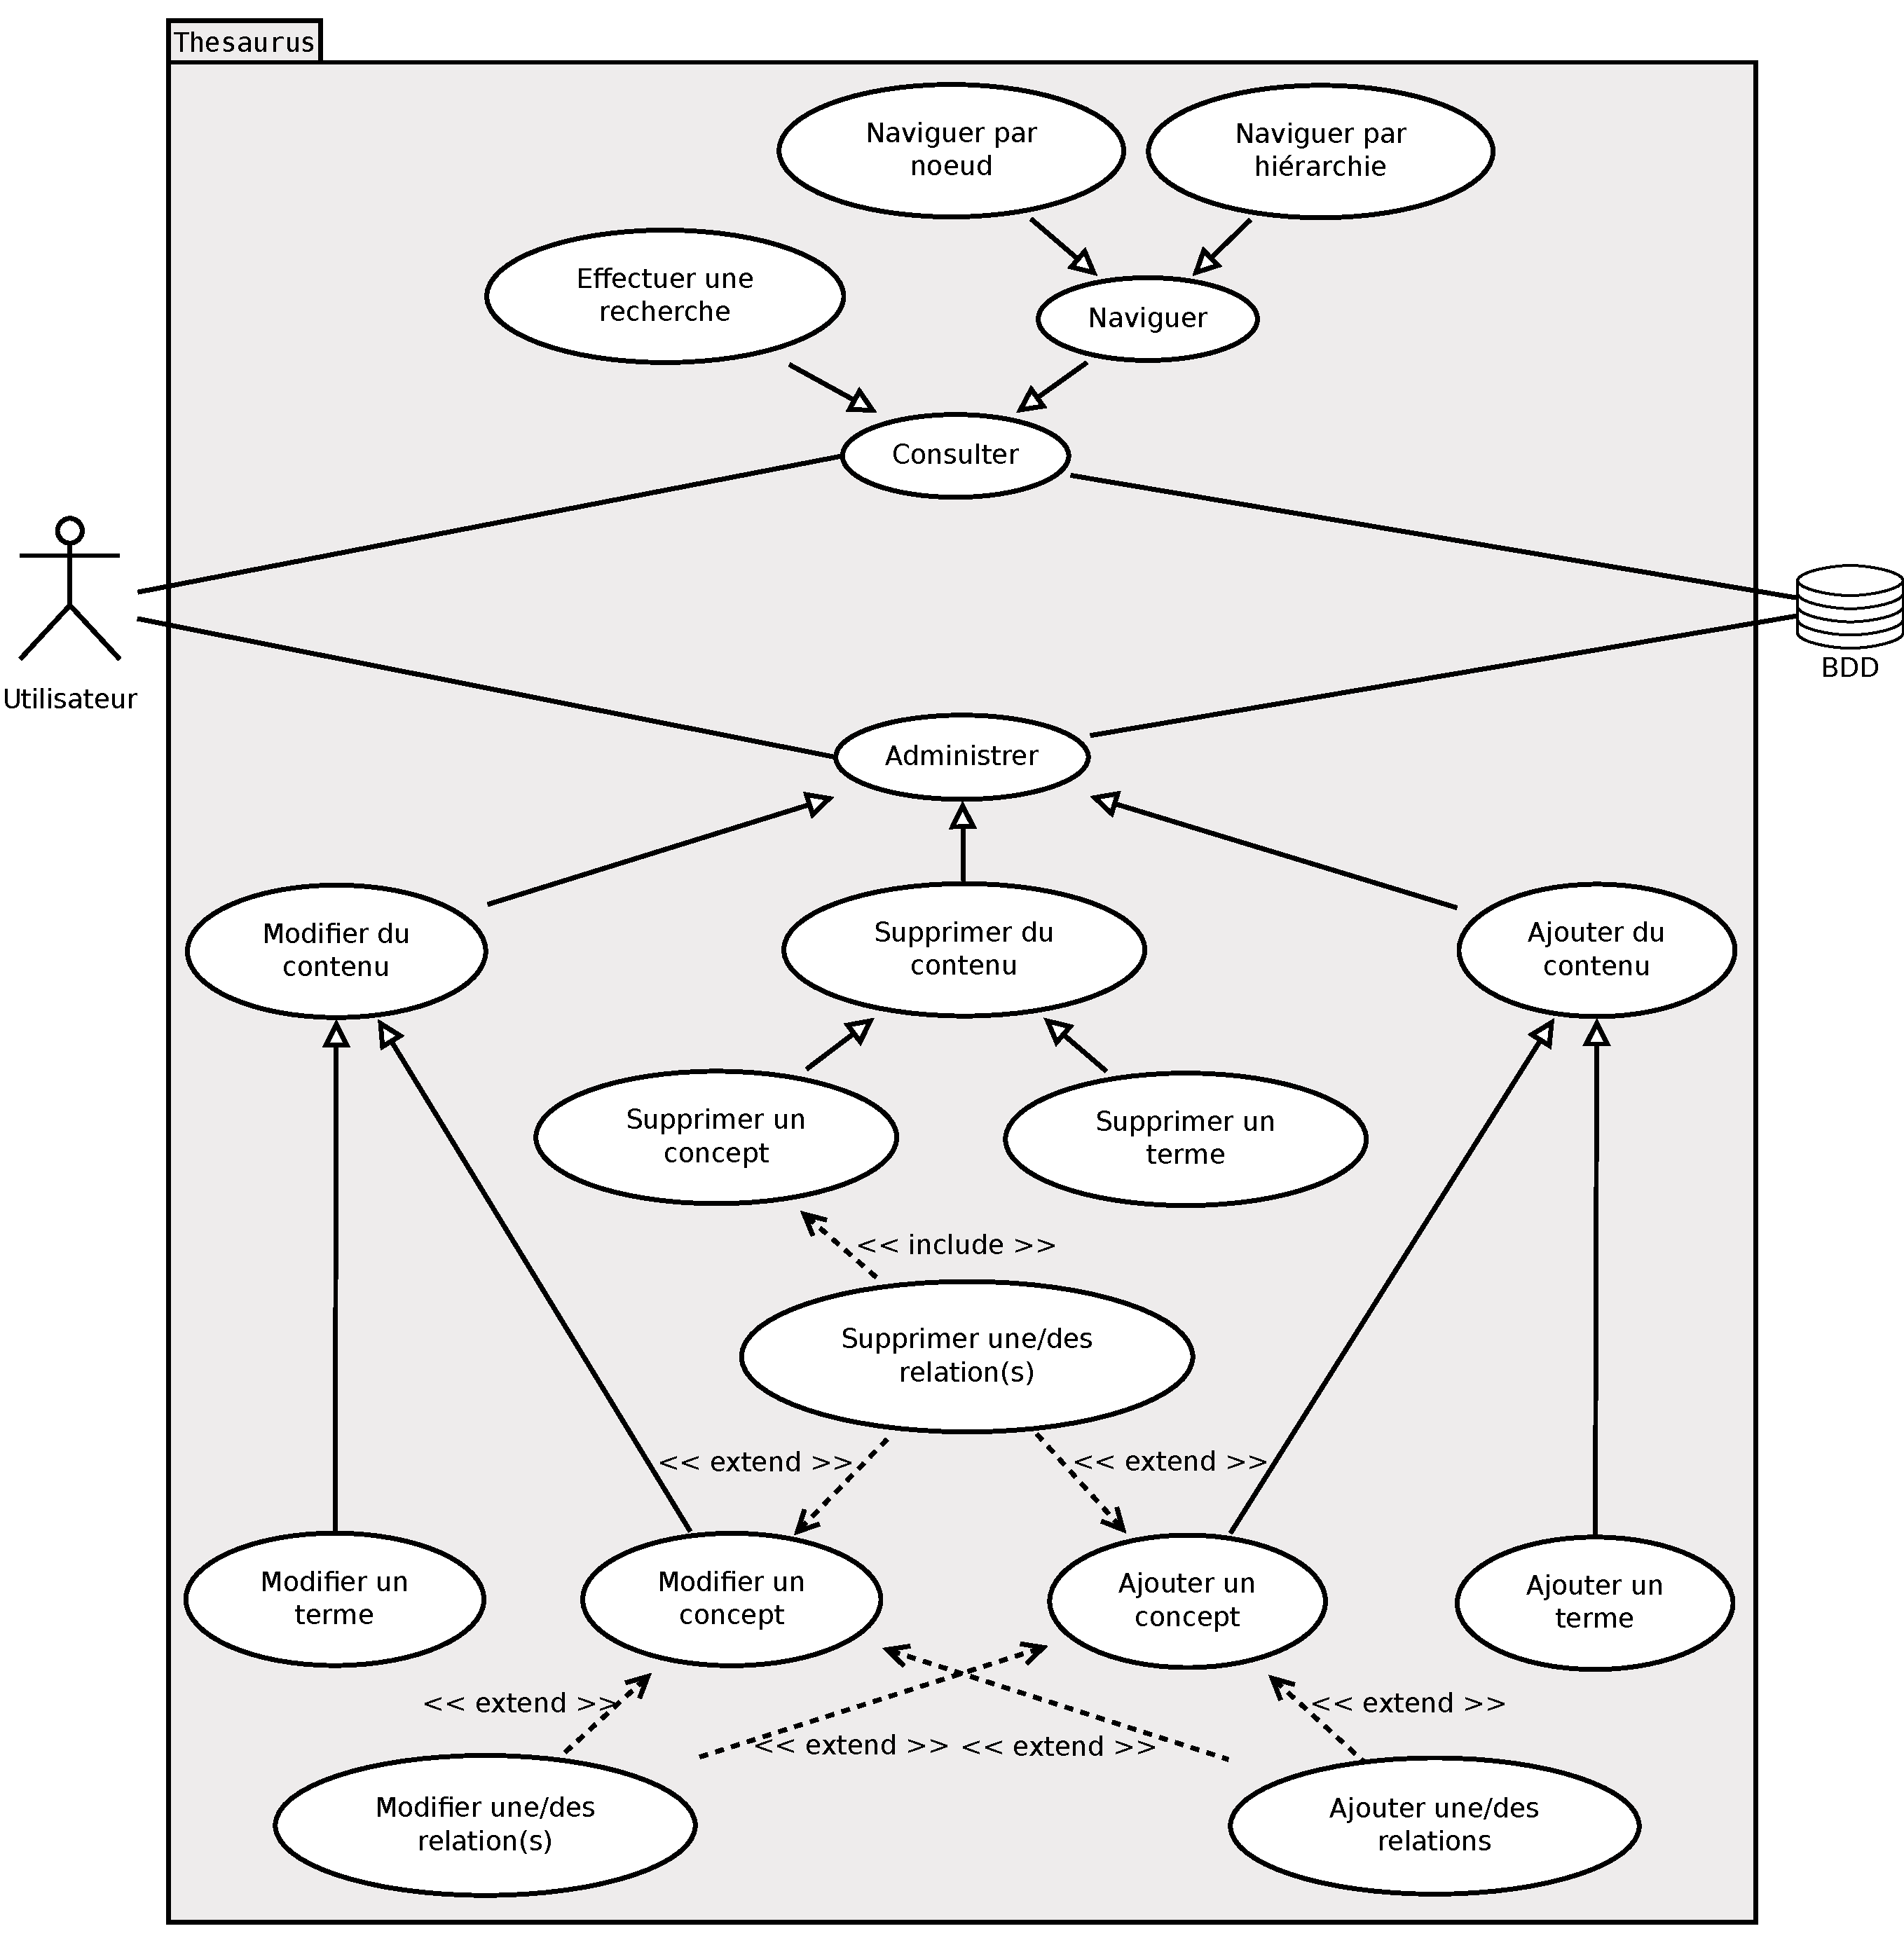
\includegraphics[width=\textwidth]{files/usecase}
\caption{Diagramme de cas d'utilisations}
\end{figure}

\section{Modélisation}
bla bla bla bla bla bla bla bla bla bla 
\subsection{Première modélisation}
bla bla bla bla bla bla 
\subsection{Évolution}
bla bla bla bla bla bla 
\subsection{Décision finale}
bla bla bla bla bla bla bla bla bla bla 